\section{Replication}

The paper by \cite{acemogluColonialOriginsComparative2001} studies the impact of colonialism on economic development. The authors employ a two-stage least squares (2SLS) approach to estimate the causal effect of early institutions on current economic performance. Specifically, they use historical data on settler mortality as an instrument for institutional quality, arguing that areas with higher settler mortality rates developed extractive institutions, which persisted and adversely affected modern economic outcomes. 

The structural relationship they estimate can be summarized as:
\begin{align*}
    \text{log GDP per capita} &= \beta \times \text{Expropriation Risk} + \varepsilon,
\end{align*}
where Expropriation Risk is instrumented by historical Settler Mortality.

The identification strategy relies on the assumption that settler mortality affects current income only through its effect on institutions, and not through other channels. In other words, settler mortality must be excluded from the structural equation for income, satisfying the exclusion restriction $\gamma = 0$.

However, this assumption has been the subject of debate. \cite{albouyColonialOriginsComparative2012} criticizes the original study by arguing that the measurement of settler mortality is problematic and that the sample of colonies used by \cite{acemogluColonialOriginsComparative2001} may introduce biases. He also points out that settler mortality could directly influence current development outcomes through channels unrelated to institutions, thereby violating the exclusion restriction.

Additionally, \cite{glaeserInstitutionsCauseGrowth2004} question the broader framework, suggesting that human capital, rather than institutions per se, may be the more fundamental driver of economic growth. If this critique holds, settler mortality could directly affect economic outcomes by shaping human capital accumulation, again violating the exclusion assumption.

Given these concerns, applying the Bayesian plausibly exogenous framework of \cite{conleyPlausiblyExogenous2012} to the \cite{acemogluColonialOriginsComparative2001} dataset provides a natural way to assess the robustness of the original findings. By allowing for a nonzero but small direct effect of settler mortality, we can explore how sensitive the estimated causal effect of institutions is to plausible violations of the exclusion restriction.

Thus, we can apply the Bayesian approach developed in the previous section to the dataset used by \cite{acemogluColonialOriginsComparative2001}. 

We specify the prior for the coefficient on the instrument ($\gamma$) with mean zero, reflecting the belief in approximate exclusion, and for the intercept term and the coefficient on the exogenous variable ($\delta$) we use the sample mean of the corresponding variable. For the prior variances, we follow the 2-$\sigma$ rule for the level coefficient and set the prior variance for the coefficient on the instrument to $10$. 

We run the Gibbs sampler for $10{,}000$ iterations, discarding the first $2{,}000$ as burn-in. The posterior summary statistics are reported in Table \ref{tab:replication_results}.


% Table created by stargazer v.5.2.3 by Marek Hlavac, Social Policy Institute. E-mail: marek.hlavac at gmail.com
% Date and time: Mon, Apr 28, 2025 - 11:55:52 PM
\begin{table}[!htbp] \centering 
  \caption{Replication Results} 
  \label{tab:replication_results} 
\begin{tabular}{@{\extracolsep{5pt}} ccccccc} 
\\[-1.8ex]\hline 
\hline \\[-1.8ex] 
Parameter & True Value & Mean & Standard Deviation & 0.025 & 0.975 & Effective Sample Size \\ 
\hline \\[-1.8ex] 
pi & -0.61 & $$-$0.58$ & $0.12$ & $$-$0.82$ & $$-$0.33$ & $6,830.29$ \\ 
phi & - & $9.21$ & $0.59$ & $8.02$ & $10.37$ & $6,751.66$ \\ 
beta & 0.94 & $0.92$ & $0.25$ & $0.50$ & $1.45$ & $13,644.54$ \\ 
gamma & 0 & $$-$0.00$ & $0.01$ & $$-$0.02$ & $0.02$ & $6,881.64$ \\ 
delta & - & $2.10$ & $1.61$ & $$-$1.40$ & $4.81$ & $13,646.41$ \\ 
\hline \\[-1.8ex] 
\end{tabular} 
\end{table} 


The true value is referencing the value of the parameter in Table 4 from \cite{acemogluColonialOriginsComparative2001}. The posterior mean and credible intervals are close to the frequentist estimates, indicating that the Bayesian model is able to recover the frequentist estimates. 

The traceplot in Figure \ref{fig:replication_traceplot} illustrates the convergence of the Gibbs sampler. We observe no discernible patterns, suggesting the Markov chain has mixed well and reached stationarity.

\begin{figure}[H]
\centering
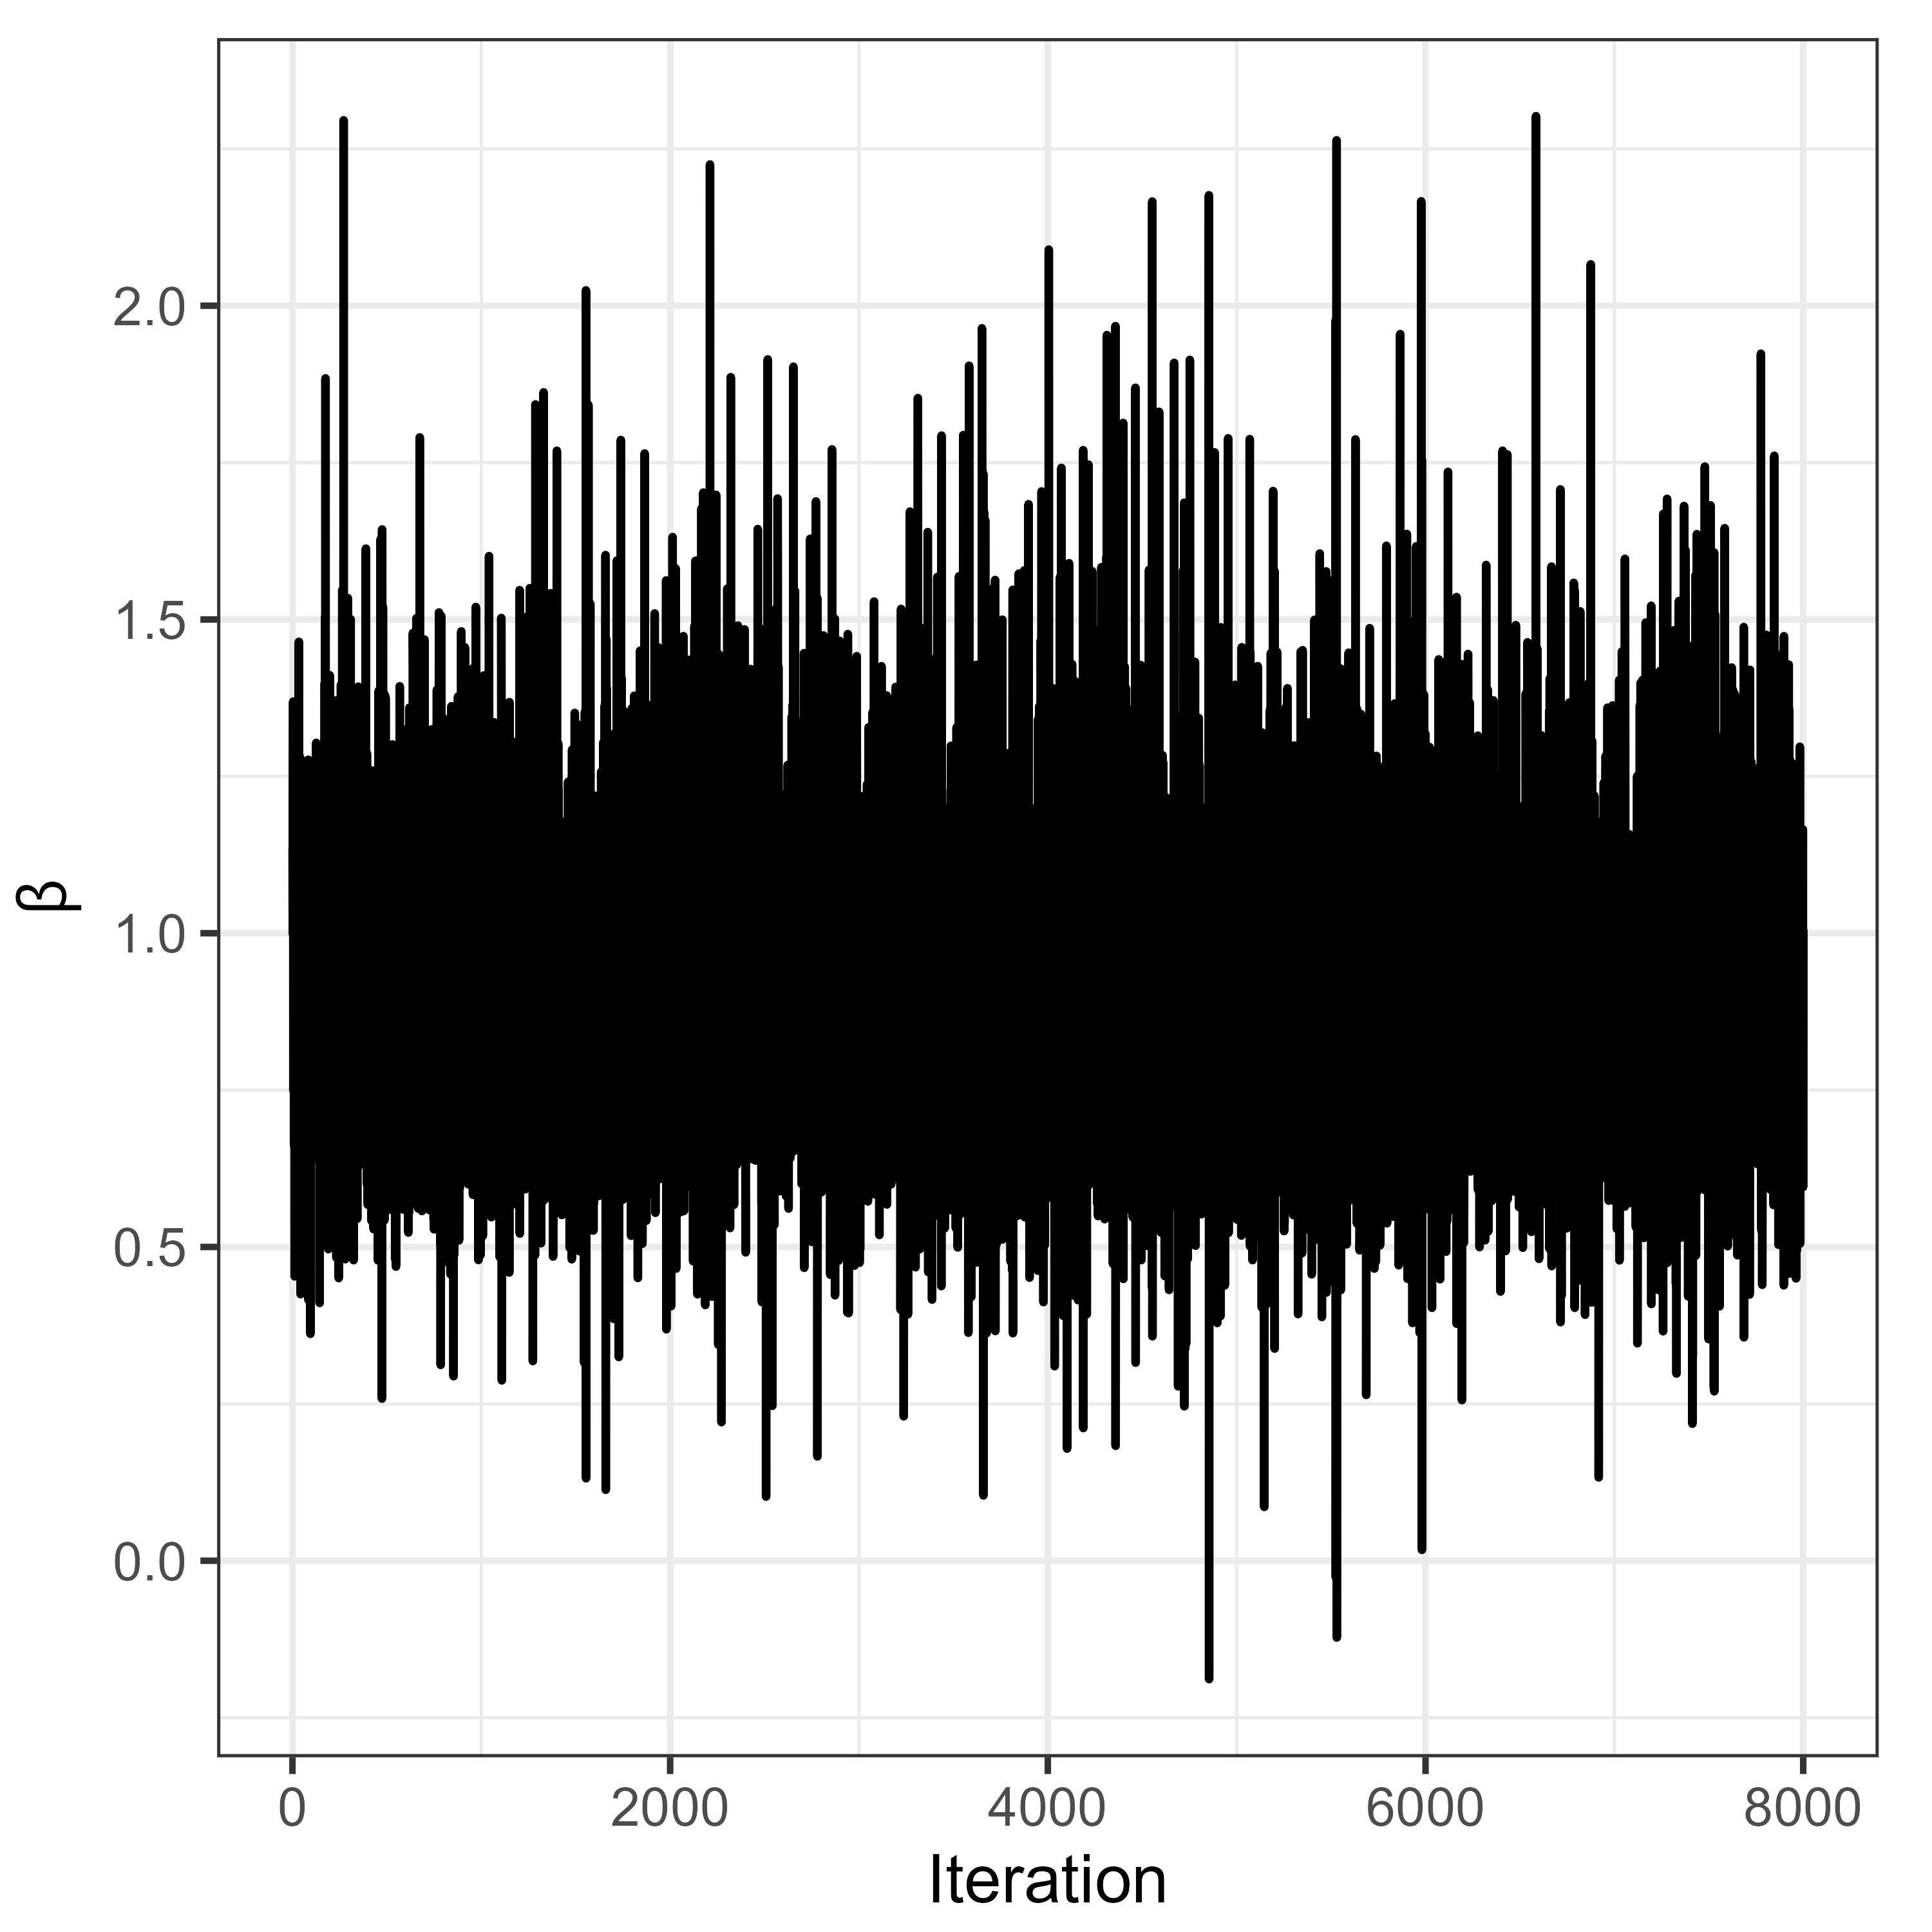
\includegraphics[width=0.8\textwidth]{../figures/acemoglu/trace_beta.png}
\caption{Traceplot of $\beta$ --- Replication Study}
\label{fig:replication_traceplot}
\end{figure}

The autocorrelation plot in Figure \ref{fig:replication_autocorrelation} shows low autocorrelation at all lags, reinforcing the evidence of good mixing and approximate independence across draws.

\begin{figure}[H]
\centering
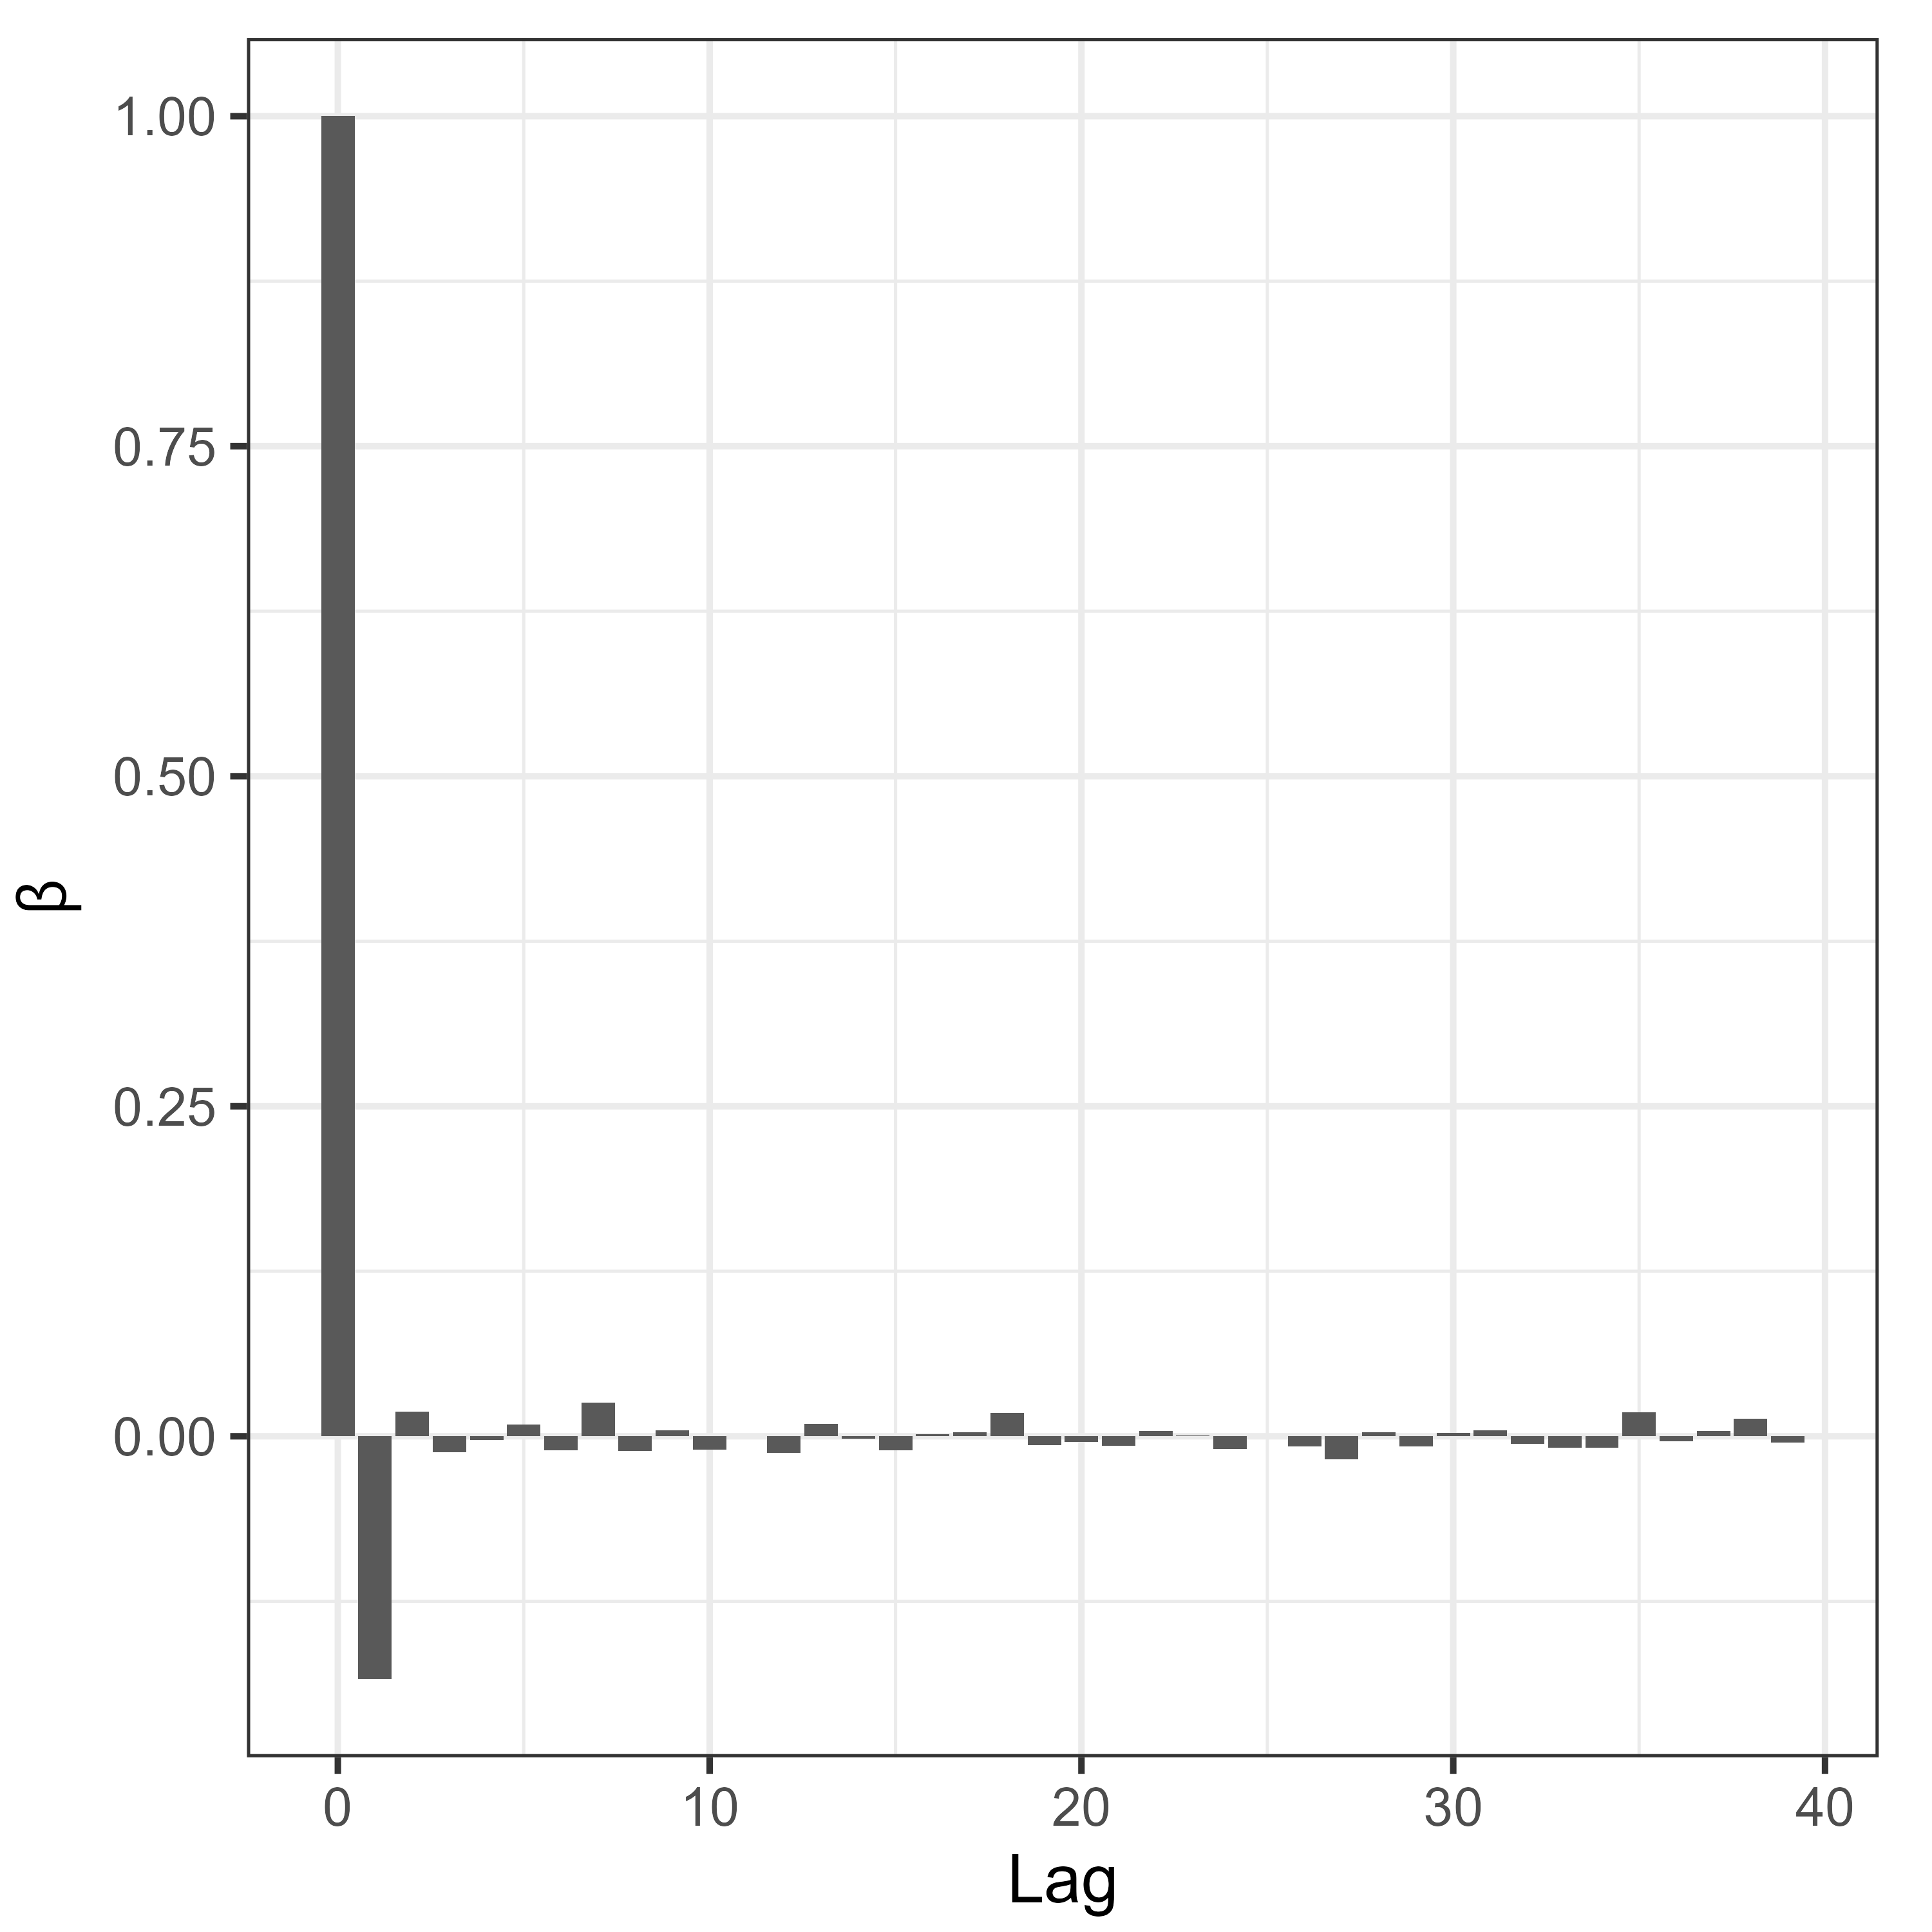
\includegraphics[width=0.8\textwidth]{../figures/acemoglu/acf_beta.png}
\caption{Autocorrelation of $\beta$ --- Replication Study}
\label{fig:replication_autocorrelation}
\end{figure}

We also present the posterior distributions of the parameters in Figure \ref{fig:replication_posterior_distributions}, visualized as histograms.

\begin{figure}[H]
\centering
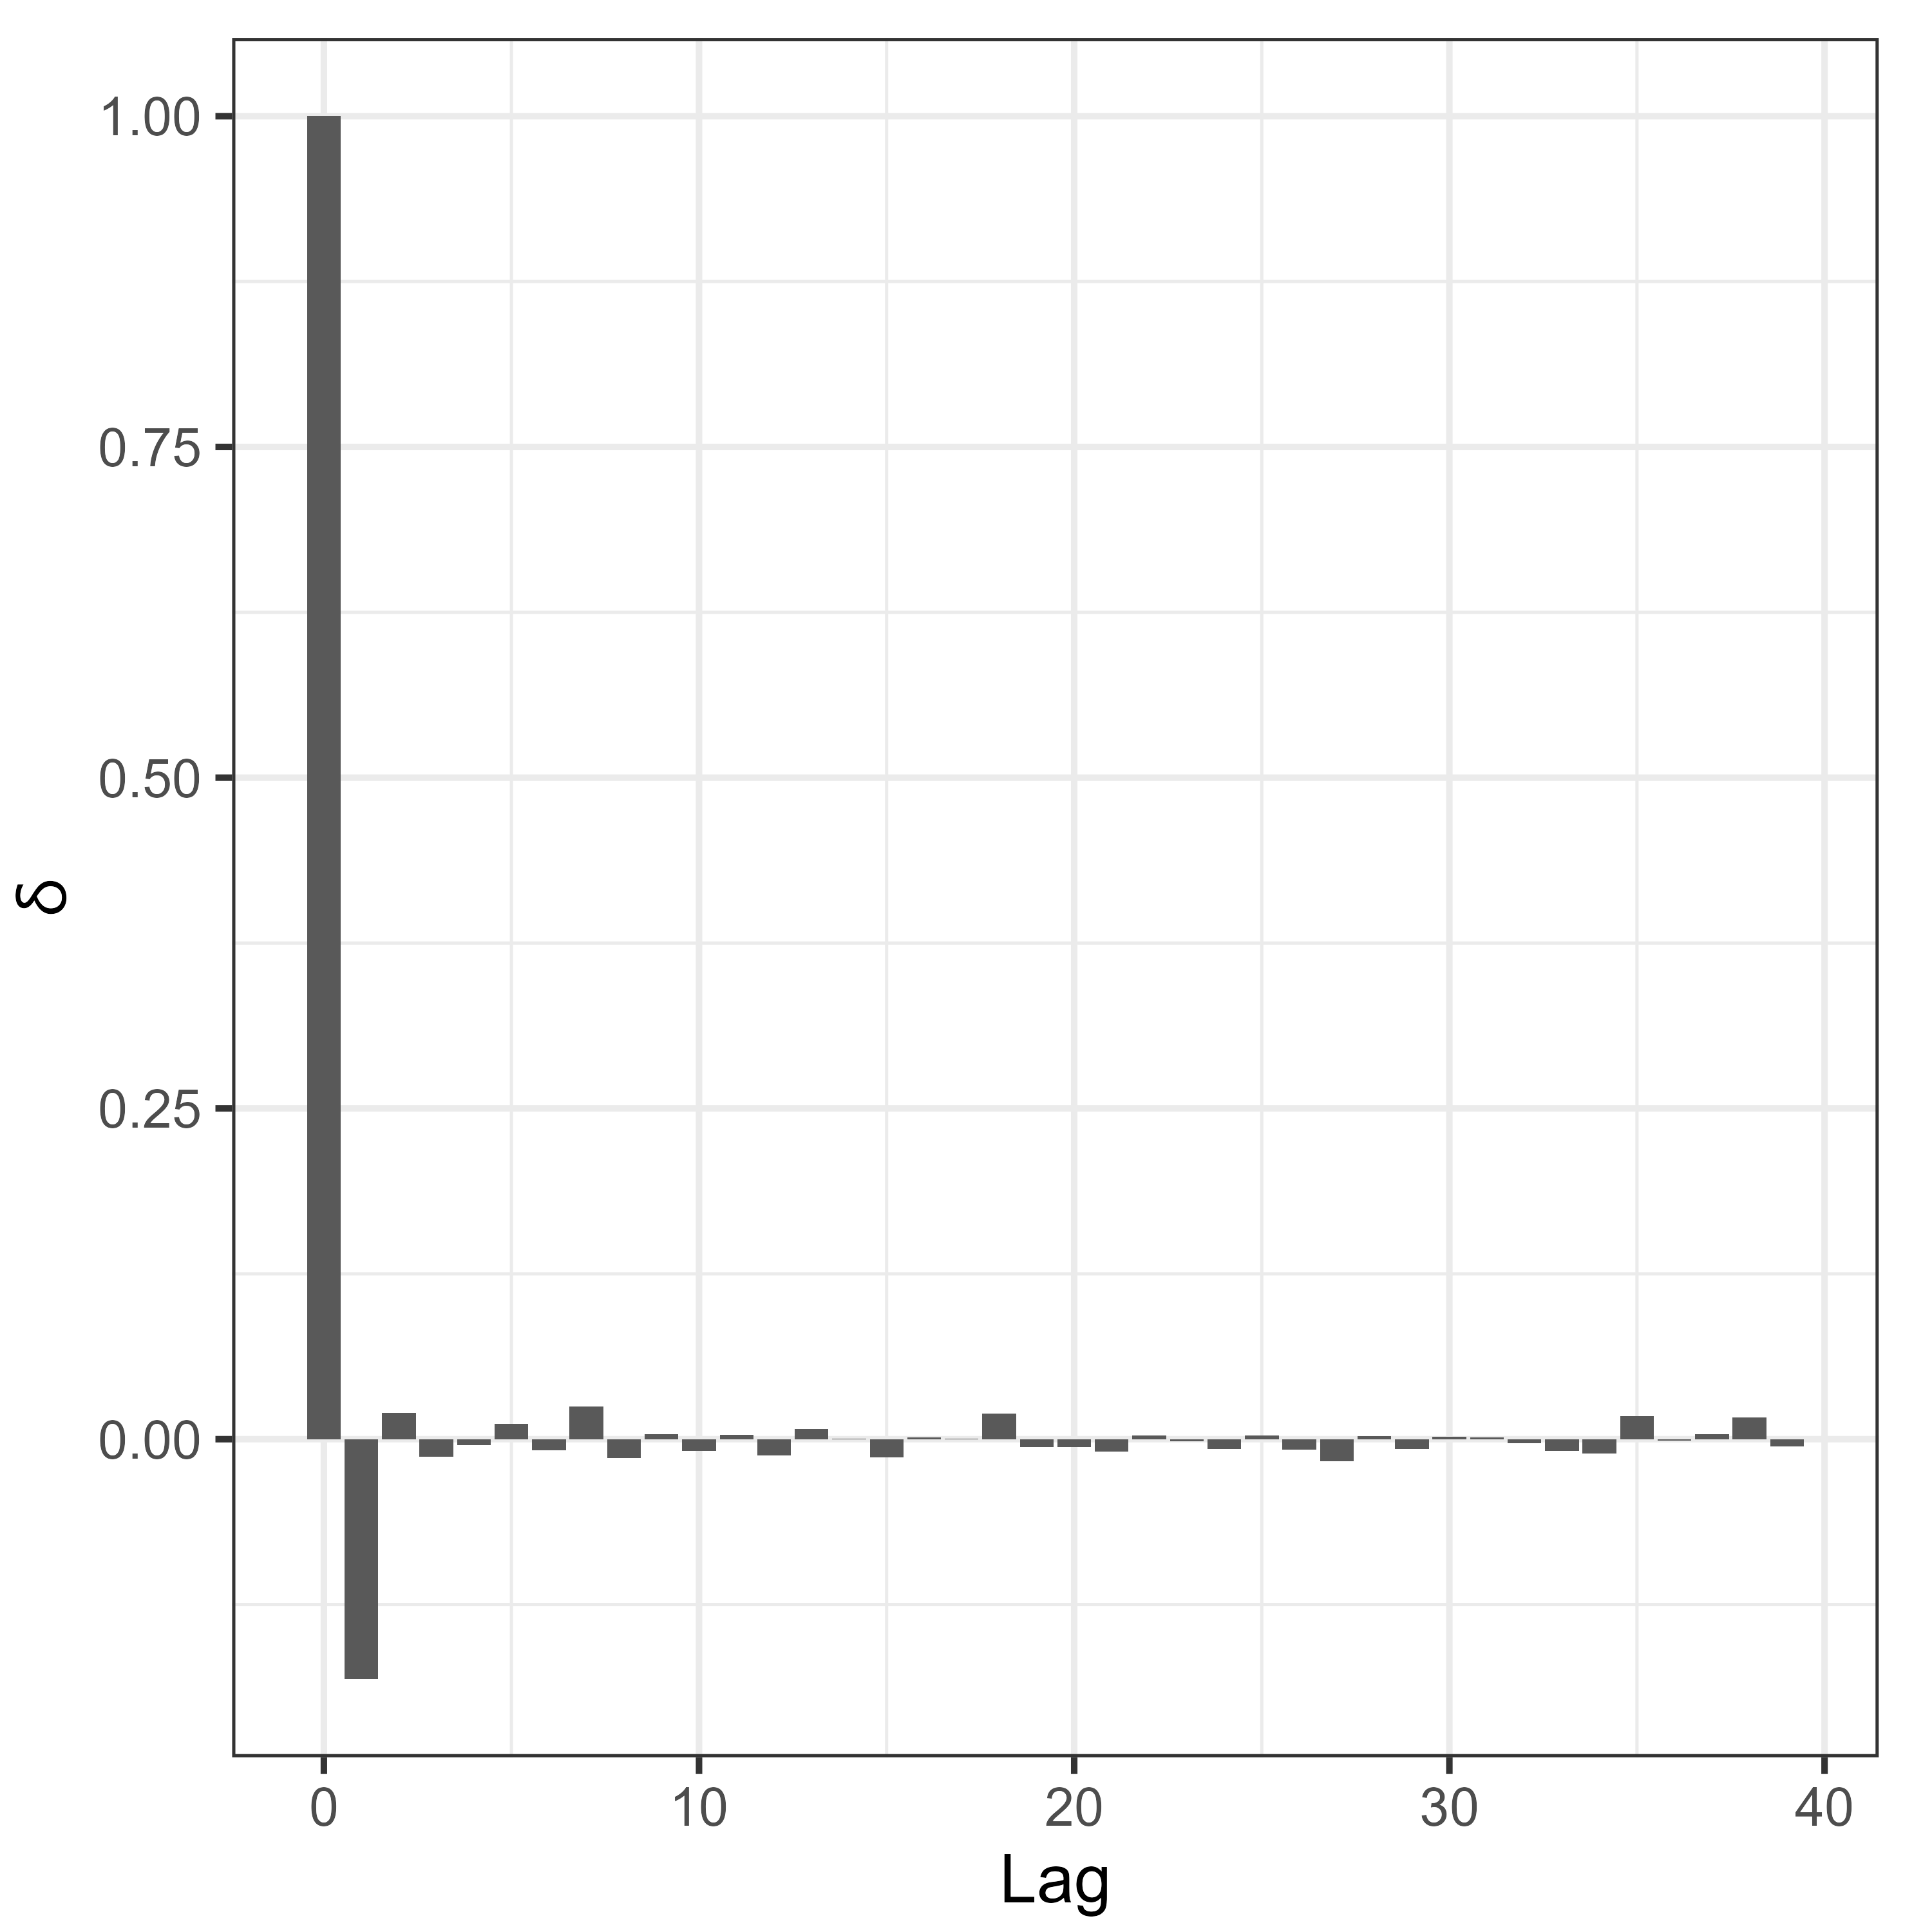
\includegraphics[width=0.8\textwidth]{../figures/acemoglu/hist_beta.png}
\caption{Posterior Distribution of $\beta$ --- Replication Study}
\label{fig:replication_posterior_distributions}
\end{figure}

As shown, our Bayesian model closely recovers the frequentist point estimates reported by \cite{acemogluColonialOriginsComparative2001} when assuming strict exclusion. This provides reassuring evidence that, under the exclusion restriction, the Bayesian and frequentist approaches align.

However, one of the main advantages of the Bayesian framework is that it naturally accommodates departures from strict exclusion. By allowing for a nonzero $\gamma$, with a prior centered at zero but with increasing variance, we can examine how the posterior inference on $\beta$ changes. 

The sensitivity analysis presented in Figure \ref{fig:replication_sensitivity_analysis} shows how varying the prior variance for $\gamma$ affects the posterior distribution of $\beta$. When the prior variance is very small, we essentially recover the frequentist estimate; as the prior variance increases, the posterior mean of $\beta$ decreases, and the credible intervals widen, reflecting increased uncertainty about the exclusion restriction.

\begin{figure}[H]
    \centering
    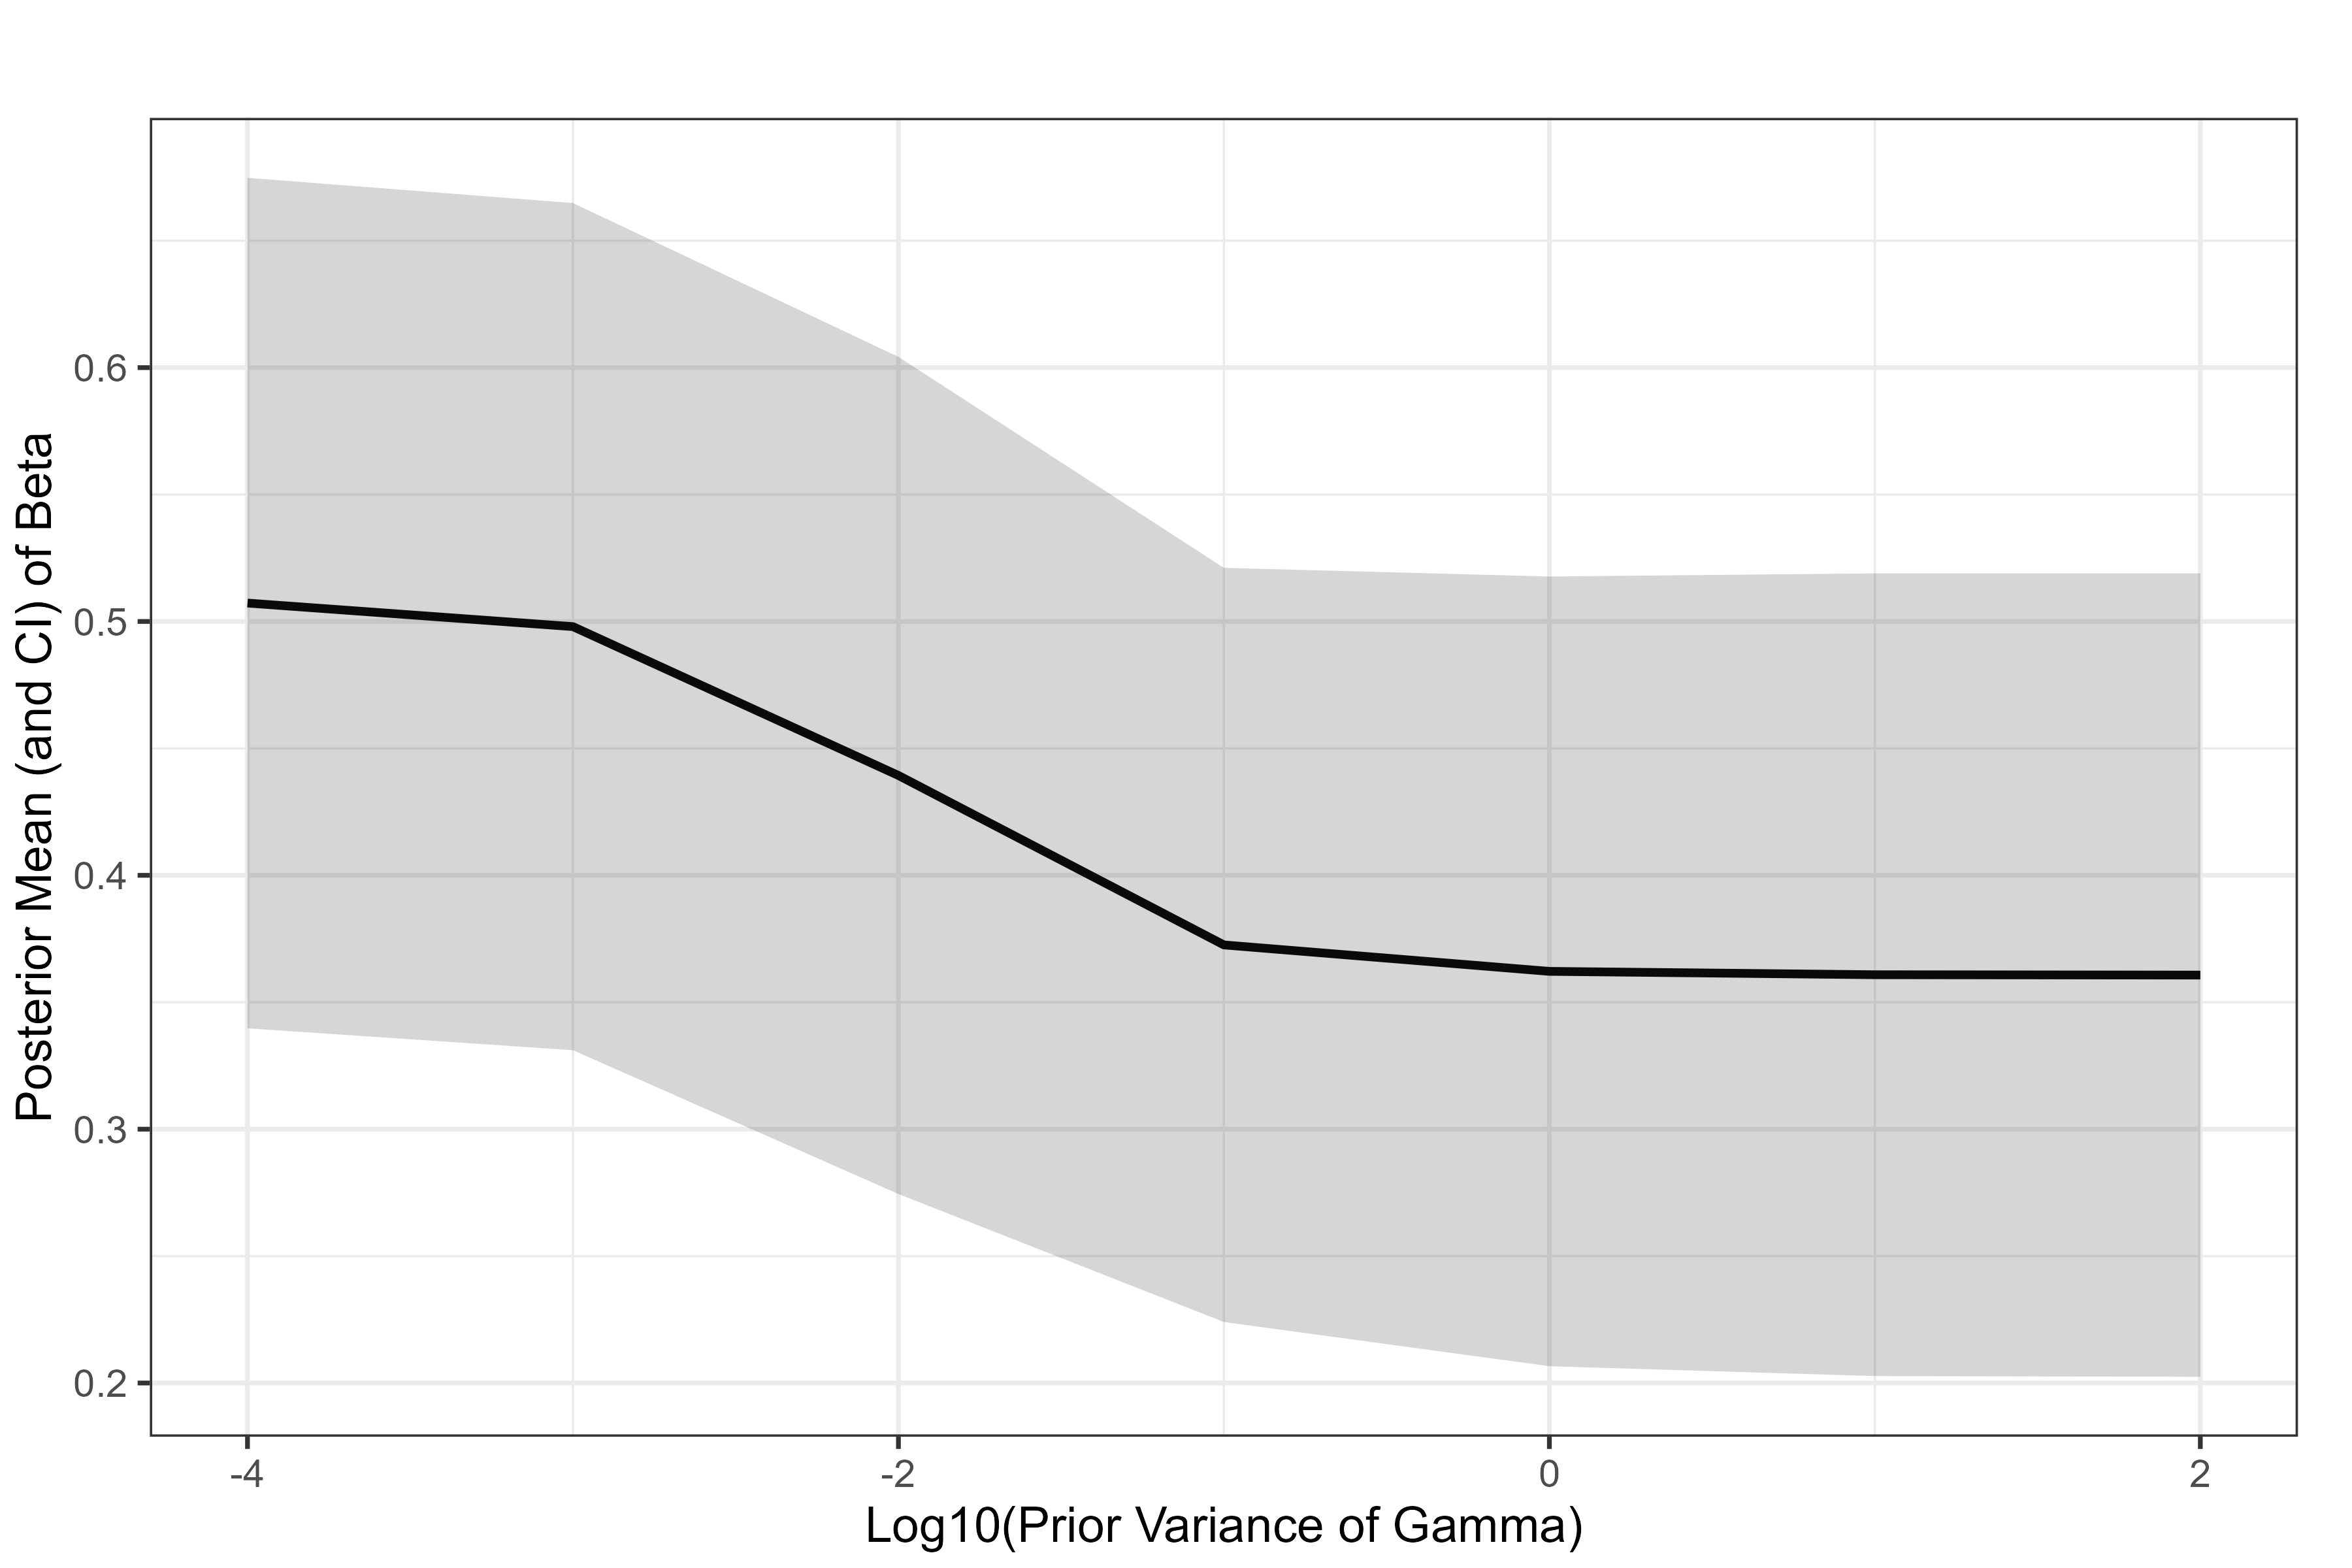
\includegraphics[width=0.9\textwidth]{../figures/acemoglu/plot_prior_gamma.png}
    \caption{Sensitivity Analysis of $\widehat{\beta}$ to Prior Variance of $\gamma$ --- Replication Study}
    \label{fig:replication_sensitivity_analysis}
    \end{figure}

It is important to note that in this specific case, even with a wide prior variance, we do not lose statistical significance of the coefficient on $\beta$. Nonetheless, in settings where significance could be lost, \cite{conleyPlausiblyExogenous2012} provide a Bayesian solution to a sensitivity analysis problem, but do not offer a direct method to incorporate the substantive expertise of the researcher regarding the likely magnitude of $\gamma$.

To address this gap, \cite{vankippersluisPlausiblyExogenous2018} propose an extension. They build upon the strategy suggested by \cite{angristWhyWorldWar1994}, who advocated examining subsamples where the first stage is weak or null. If the exclusion restriction holds, the reduced form should also show no significant relationship in these subsamples. 

\cite{vankippersluisPlausiblyExogenous2018} adapt this idea to the Bayesian framework: for observations where the first-stage effect is weak, they use the estimated reduced form coefficient to inform a prior for the direct effect $\gamma$. If the reduced form in such subsamples is significantly different from zero, it suggests a violation of exclusion, and this information is incorporated into the prior for $\gamma$.

However, this approach requires assuming homogeneous treatment effects, even though heterogeneous effects are likely present, particularly when the first-stage relationship varies across subsamples. Additionally, selecting the appropriate subsample is nontrivial and must be done carefully to avoid introducing further biases.

\bigskip

In summary, we review the approaches of \cite{conleyPlausiblyExogenous2012} and \cite{vankippersluisPlausiblyExogenous2018} to account for possible violations of the exclusion restriction within a Bayesian framework. We apply these methods to simulated datasets and to the empirical context of \cite{acemogluColonialOriginsComparative2001}. We find that the Bayesian plausibly exogenous approach not only recovers the frequentist estimates under strict exclusion but also provides a powerful and flexible tool for sensitivity analysis when the validity of the instrument is questionable.
